\documentclass[sigconf, authorversion, review]{acmart}

\usepackage{booktabs} % For formal tables

% TOG prefers author-name bib system with square brackets
\citestyle{acmauthoryear}
\setcitestyle{square}


\usepackage[ruled]{algorithm2e} % For algorithms
\renewcommand{\algorithmcfname}{ALGORITHM}
\SetAlFnt{\small}
\SetAlCapFnt{\small}
\SetAlCapNameFnt{\small}
\SetAlCapHSkip{0pt}
\IncMargin{-\parindent}


%% My stuff
\DeclareMathOperator*{\argmin}{arg\,min}

% Metadata Information
\acmJournal{TOG}
\acmVolume{9}
\acmNumber{4}
\acmArticle{39}
\acmYear{2018}
\acmMonth{3}

% Copyright
%\setcopyright{acmcopyright}
%\setcopyright{acmlicensed}
%\setcopyright{rightsretained}
%\setcopyright{usgov}
\setcopyright{usgovmixed}
%\setcopyright{cagov}
%\setcopyright{cagovmixed}

% DOI
\acmDOI{0000001.0000001_2}

% Paper history
\received{February 2007}
\received{March 2009}
\received[final version]{June 2009}
\received[accepted]{July 2009}


% Document starts
\begin{document}
% Title portion
\title{Interactive Stress Analysis via Nonlinear Subspace Simulation}

\author{Lawson Fulton, David I.W. Levin, David Duvenaud, Alec Jacobson}
\orcid{0000-0001-7281-8117}
%\affiliation{%
% \institution{University of Toronto}
% \streetaddress{40 St. George Street}
% \city{Toronto}
% \state{ON}
% \postcode{M5S 2E4}
% \country{Canada}
% }
%\author{David I.W. Levin}
%\orcid{0000-0002-5043-8698} % chktex 8
%\affiliation{%
% \institution{University of Toronto}
% \streetaddress{40 St. George Street}
% \city{Toronto}
% \state{ON}
% \postcode{M5S 2E4}
% \country{Canada}
% }
%\author{David Duvenaud}
%\affiliation{%
% \institution{University of Toronto}
% \streetaddress{40 St. George Street}
% \city{Toronto}
% \state{ON}
% \postcode{M5S 2E4}
% \country{Canada}
% }
%\author{Alec Jacobson}
\affiliation{%
 \institution{University of Toronto}
 \streetaddress{40 St. George Street}
 \city{Toronto}
 \state{ON}
 \postcode{M5S 2E4}
 \country{Canada}
 }

\renewcommand\shortauthors{Fulton, L. et al}

%\begin{abstract}
%\end{abstract}


%
% The code below should be generated by the tool at
% http://dl.acm.org/ccs.cfm
% Please copy and paste the code instead of the example below.
%
\begin{CCSXML}
    <ccs2012>
        <concept>
            <concept_id>10002944.10011123.10011673</concept_id>concept_id>
            <concept_desc>General and reference~Design</concept_desc>concept_desc>
            <concept_significance>500</concept_significance>concept_significance>
        </concept>concept>
        <concept>
            <concept_id>10010147.10010371.10010352.10010379</concept_id>concept_id>
            <concept_desc>Computing methodologies~Physical
            simulation</concept_desc>concept_desc>
            <concept_significance>500</concept_significance>concept_significance>
        </concept>concept>
        <concept>
            <concept_id>10010147.10010371.10010396.10010397</concept_id>concept_id>
            <concept_desc>Computing methodologies~Mesh
            models</concept_desc>concept_desc>
            <concept_significance>300</concept_significance>concept_significance>
        </concept>concept>
    </ccs2012>ccs2012>
\end{CCSXML}

\ccsdesc[500]{General and reference~Design}
\ccsdesc[500]{Computing methodologies~Physical simulation}
\ccsdesc[300]{Computing methodologies~Mesh models}

%
% End generated code
%

\keywords{simulation, machine learning}

\begin{teaserfigure}
  \centering
  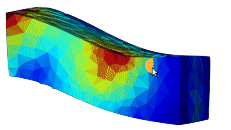
\includegraphics[width=.3\textwidth]{figures/teaser}\hspace{2cm}
    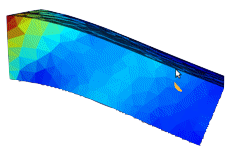
\includegraphics[width=.3\textwidth]{figures/teaser2}
  \caption{Real time stress field visualization of a 2k vertex model at 20ms/frame\label{fig:teaser}}
\end{teaserfigure}

\maketitle

%%%%%%%%%%%%%%%%%%%%%%%%%%%%%%%%%%%%%%%%%%%%%%%%%%%%%%%%%%%%%%%%%%%%%%%%%%%%%%%%
\section{Introduction}\label{sec:intro}
Predicting the stress experienced by physically simulated objects intended for manufacturing is an important step of the design process. However, the complex finite element simulations required to accurately perform this task are often too slow for real-time feedback.

Because of this, there has been decades of work attempting to accelerate solid mechanics simulations for the purposes of stress analysis. Such works take two broad forms, solver-based approaches (which attempt to improve the linear algebraic operations at the heart of a physics simulator) or discretization-based approaches (which try to reduce the degrees-of-freedom) in a computational mesh. One of the most successful techniques for speeding up simulations is linear modal analysis, a discretization-based method which performs simulation in a small linear reduced space constructed from the linear deformation modes of an object. 

However, linear modal analysis has issues which prevent it from being a panacea to the performance problems of physics-based simulation. First, anything beyond the linear modes can be difficult to compute, relying on non-linear modal derivatives. Second, motions which span highly non-linear regions of the configuration space can require large linear spaces to accurately represent. This can have a dire impact on runtimes, since system matrices for small reduced spaces become dense and even a small increase in the number of modes can have a hampering effect on performance. Existing fast integration schemes for reduced models typically have $O(r^2)$ to $O(r^4)$ asymptotic behavior where $r$ is the dimension of the reduced space as in \cite{Barbic-05} .

Ideally, one would generate as small a reduced space as necessary directly from simulation data. A strictly linear basis can make this difficult. In this paper we flaunt conventional wisdom and disregard linearity, in favor of non-liner dimensionality reduction techniques. In particular we draw from the field of machine learning and devise a new autoencoder architecture that can efficiently represent non-linear deformations with high fidelity using fewer degrees of freedom than a corresponding linear reduced representation. Furthermore we develop a minimization based time integrator that takes advantage of our reduced representation to produce dynamic simulations of production quality meshes at interactive rates.



%%%%%%%%%%%%%%%%%%%%%%%%%%%%%%%%%%%%%%%%%%%%%%%%%%%%%%%%%%%%%%%%%%%%%%%%%%%%%%%%
\section{Related Work}\label{sec:related}


There have been several attempts in recent literature to speed up stress analysis for shape design through pre-computation.
% Head 2
\subsection{Sampling and Interpolation}

The approach used in \cite{Schulz-17} is to do a full stress analysis at multiple points within the parameter space, and use a clever interpolation scheme to produce intermediary results. This approach has the benefit of handling varying mesh topologies, but requires storing $2^k$ meshes where $k$ is the number of model parameters, thus requiring large amounts of storage for complex designs.

% Head 3
\subsection{Reduced Space Computation}

Another approach, as in \cite{Chen-16}, is to use a small linear basis to generate the stress field and do a complete solve within this reduced space. This approach avoids storage of meshes, but has the drawback of only working for fixed mesh topologies. Therefore it is unsuitable for typical CAD models which have varying mesh topologies for each choice of design parameters.

For large deformations, linear subspace integration techniques such as \cite{Barbic-05} and \cite{vonTycowicz-13} can also be used.

Traditionally, subspace simulation proceeds by constructing an orthonormal basis matrix $U\in M^{r\times n}$ where $n$ is the total number of degrees of freedom in the system, and $r$ is the size of the reduced space. Then the mapping from the reduced to the full space can be written as
$$q^t=U^Tz^t$$

Their are multiple approaches for constructing $U$, such as computing the linear deformation modes, or performing principle component analysis (PCA) on simulation snapshots. However, they all suffer from the same fundamental drawback of requiring a large number of bases to represent significant non-linear deformations.

\subsection{Machine Learning Approaches}
We are not the first to propose machine learning driven approach to physical simulation. In \cite{Ladicky-15} and \cite{CNNFluid2016}, they propose models to explicitly predict the solution of the systems.

\subsection{Simulation as Optimization}
Several authors have proposed minimization schemes for optimization such as \cite{Liu-17} and \cite{Wang-16}.


%%%%%%%%%%%%%%%%%%%%%%%%%%%%%%%%%%%%%%%%%%%%%%%%%%%%%%%%%%%%%%%%%%%%%%%%%%%%%%%%
\section{Methods}
Our approach is to create a reduced space representation of our system with as few degrees of freedom as possible while maintaining deformation fidelity. In \cite{Musialski-16}, they show that shrinking the size of the reduced space leads to far fewer gradient descent iterations during optimization. 

\subsection{Subspace Construction}
%TODO: Make a figure demonstrating my network architecture.\\
Our goal is to create a reduced space mapping that can capture large non-linear deformations with few degrees of freedom. One way to represent such a mapping is to use an artificial neural network. In particular, to facilitate the training of our network, we use a fully connected autoencoder trained with a mean squared error (MSE) loss.
$$L_\theta(x)=||D_\theta(E_\theta(x)) - x||^2$$

Where $D_\theta:\mathbb{R}^r\to\mathbb{R}^n$ is the decoder network, and $E_\theta:\mathbb{R}^n\to\mathbb{R}^r$ is the encoder network and $\theta$ are the network parameters. Each network is defined by a sequence of fully connected layers of rectified linear units (RELU) varying widths. A single layer $i$ has the form
$$D^i(x)=\max(W^i x - b^i, 0)$$
and the full decoder network of $l$ layers is then
$$D(x)=D^l\circ D^{(l-1)}\circ \dots \circ D^0(x)$$

We train this autoencoder using a form of stochastic gradient descent known as ADAM \cite{adam} on a collection of example displacements generated from a full space simulation for a particular model.

As a consequence of our MSE loss, we found that our network had difficulty converging to a smooth representation in its unmodified form. Our solution was to initialize the first and last layers of our autoencoder with weights obtained from performing PCA on the training data. The number of components used to perform the PCA was chosen such that the training data could be recovered with an MSE of less than $10^{-3}$. Allowing the weights of the PCA layers to learn further did not improve convergence, and significantly slowed the rate of learning, hence we chose to fix them during training. A comparison of results from our PCA-autoencoder with a plain autoencoder can be seen in figure ~\ref{fig:noisy}. 

\begin{figure}[ht!]
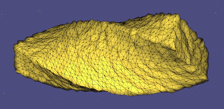
\includegraphics[width=.35\textwidth]{figures/noisy-bar}\hfill
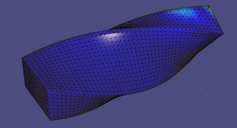
\includegraphics[width=.35\textwidth]{figures/smooth-bar}
\caption{A comparison of the decoded representation without (top) and with (bottom) PCA initialized outer layers.}
\label{fig:noisy}
\end{figure}

Through experiment we found that two fully connected layers of 200 units between the PCA and encoded layer worked well. Increasing the number of layers or number of nodes past this point did not improve the converged error on our examples.

%TODO show convergence plots of training.



\subsection{Equations of Motion}
In order to take advantage of our reduced representation, it is useful to formulate our simulation as an implicit integration scheme based on minimization in the reduced space. We derive our update scheme from Gauss' principle of least constraint, which formulates the equations of motion as a minimization over the instantaneous acceleration $a$
$$a=\argmin_a{\frac{1}{2}(Ma-F)^TM^{-1}(Ma-F)}$$

We proceed to discretize in time
$$a=\frac{v^{t+1}-v^t}{h}=\frac{q^{t+1}-2q^{t}+q^{t-1}}{h^2}$$

and then computing the next configuration $q^{t+1}$ is given by
\begin{multline}
q^{t+1}=\argmin_{q^{t+1}}\frac{1}{2h^2}(q^{t+1}-2q^{t}+q^{t-1})^TM(q^{t+1}-2q^{t}+q^{t-1})\\-\frac{1}{h}(v^{t+1}-v^t)^TF(q^{t+1})
\end{multline}

The force term in (1) can be seen as the work done by the body forces over the timestep and the external forces.
$$-\frac{1}{h}(v^{t+1}-v^t)^TF(q^{t+1})=h\Psi(q^{t+1})-h(v^{t+1}-v^t)^TF_{\mathrm{ext}}$$
Where $\Psi(q^t)$ gives the deformation energy at the given configuration. We use a standard Neo-Hookean elasticity energy.
The final update formula then becomes
%$\mathbf{TODO}$  Explain the changing $h$s..
\begin{multline}
q^{t+1}=\argmin_{q^{t+1}}\frac{1}{2}(q^{t+1}-2q^{t}+q^{t-1})^TM(q^{t+1}-2q^{t}+q^{t-1})\\+h^2[\Psi(q^{t+1})-(q^{t+1}-2q^{t}+q^{t-1})^TF_{\mathrm{ext}}]
\end{multline}

and the gradient is given by
$$\frac{\partial L}{\partial q^{t+1}} = M(q^{t+1}-2q^{t}+q^{t-1}) - hF_{\mathrm{int}}(q^{t+1})-hF_{\mathrm{ext}}$$

If we are performing the optimization within the constraints of a reduced space, then we let $q^t=D(z^t)$ where $D$ is the mapping from our reduced coordinate configuration $z$ to the full configuration $q$. And then our gradient simply becomes
$$\frac{\partial L}{\partial z^{t+1}} = J_{t+1}^T[M(q^{t+1}-2q^{t}+q^{t-1}) - hF_{\mathrm{int}}(q^{t+1})-hF_{\mathrm{ext}}]$$
Where $J_{t+1}$ is the jacobian matrix of our reduced space.
$$J_{t+1} = \frac{\partial D}{\partial z}|_z^{t+1}$$

\subsection{Optimization}

Our formulation of the simulation update as a minimization problem is naturally suited to Quasi-Newton methods such as L-BFGS (Limited memory Broyden-Fletcher-Goldfarb-Shanno algorithm)\cite{Byrd1994}. A similar approach is employed by \cite{Liu-17} and \cite{Wang-16}.

The main challenge when using this gradient descent approach with our neural network reduced space is the requirement for the network jacobian. In our examples we use finite differences to compute the jacobian because of technical limitations of our machine learning framework tensorflow. However, because our reduced space is small, this does not pose a significant performance disadvantage. In future work we hope to implement analytical jacobian calculation.

Another issue we encountered was lack of convergence in that autoencoder space. To combat this, we fixed the maximum L-BFGS iteration count to 5. This provided satisfactory performance.

\subsection{Stress Analysis}
For the stress analysis and visualization, we compute the von Mises stress from the Cauchy stress computed in the full space.

%%%%%%%%%%%%%%%%%%%%%%%%%%%%%%%%%%%%%%%%%%%%%%%%%%%%%%%%%%%%%%%%%%%%%%%%%%%%%%%%
\section{Results and Discusion}
For performance comparison we ran our simulation on a 1908 vertex bar fixed at one end. The Young's modulus was set to $3\times10^5$ and the Poisson's ration to $0.45$.

\begin{figure}[ht!]
\begin{center}
    \begin{tabular}{| l | l | l | l |}
    \hline
    Method & \# DOF & Step speed & Quality \\ \hline
    Full space & 1908 & 500ms & No distortion \\ \hline
    Linear space & 10 & 30-40ms & Minimal distortion \\ \hline
    Linear space & 3 & 15-25ms & Large distortion \\ \hline
    $\mathbf{Autoencoder}$ & $\mathbf{3}$ & $\mathbf{20-30ms}$ & $\mathbf{Some\ distortion}$ \\
    \hline
    \end{tabular}
\end{center}
\caption{A comparison of the performance of various reduced spaces.}
\label{fig:results-table}
\end{figure}

In figure ~\ref{fig:distortion} one can see the inaccurate stress field results produced by using too few degrees of freedom in a linear space.

\begin{figure}[ht!]
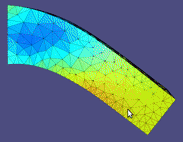
\includegraphics[width=.25\textwidth]{figures/distortion-example}
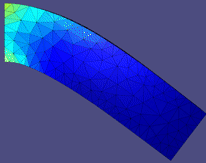
\includegraphics[width=.25\textwidth]{figures/no-distortion-full}\hfill
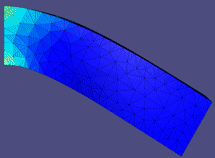
\includegraphics[width=.25\textwidth]{figures/no-distortion-ae}
\caption{Top: 3dof PCA subspace, Middle: Full space, Bottom: 3dof Autoencoder space }
\label{fig:distortion}
\end{figure}

%%%%%%%%%%%%%%%%%%%%%%%%%%%%%%%%%%%%%%%%%%%%%%%%%%%%%%%%%%%%%%%%%%%%%%%%%%%%%%%%
\section{Conclusion}\label{sec:conclusion}
We have demonstrated the effectiveness of non-linear subspace simulation for real time stress field analysis. With our unoptimized implementation, we are able to match state of the art results in linear subspace simulation using far fewer degrees of freedom.

\subsection{Limitations and Future Work}
The quality of the reduced space learned by our autoencoder is still one of the primary issues. We hope that by implementing dynamics aware regularization into the training process we will produce smoother mappings and improve the performance of the L-BFGS convergence.

We also hope to do away with finite differences and efficiently compute the analytical jacobian of our decoder.

% \begin{acks}
% \end{acks}

%%%%%%%%%%%%%%%%%%%%%%%%%%%%%%%%%%%%%%%%%%%%%%%%%%%%%%%%%%%%%%%%%%%%%%%%%%%%%%%%
\bibliographystyle{ACM-Reference-Format}
\bibliography{final-paper}

\end{document}
